\documentclass[twocolumn]{jsarticle}
%
\usepackage{amsmath,amssymb}
\usepackage{bm}
\usepackage{graphicx}
\usepackage{ascmac}
\usepackage{subfigure}
\usepackage{multicol}
\usepackage{setspace}
\usepackage{url}
%
\setlength{\textwidth}{\fullwidth}
\setlength{\textheight}{39\baselineskip}
\addtolength{\textheight}{\topskip}
\setlength{\voffset}{-0.5in}
\setlength{\headsep}{0.3in}
%
\newcommand{\divergence}{\mathrm{div}\,}  %ダイバージェンス
\newcommand{\grad}{\mathrm{grad}\,}  %グラディエント
\newcommand{\rot}{\mathrm{rot}\,}  %ローテーション
\renewcommand{\baselinestretch}{1}
\renewcommand{\figurename}{Fig.}
\renewcommand{\tablename}{Table.}

\newcommand{\bi}{\bfseries\itshape}
\newcommand{\bq}{\begin{equation}}
\newcommand{\eq}{\end{equation}}
\newcommand{\bn}{\vspace{-2mm}\begin{eqnarray}}
\newcommand{\en}{\vspace{-2mm}\end{eqnarray}}
\newcommand{\ba}{\begin{array}}
\newcommand{\ea}{\end{array}}
\newcommand{\lt}{\left}
\newcommand{\rt}{\right}
\newcommand{\bc}{\begin{center}}                            %%% 中央揃え
\newcommand{\ec}{\end{center}}
\newcommand{\bfr}{\begin{flushright}}                       %%% 右揃え
\newcommand{\efr}{\end{flushright}}
\newcommand{\beqa}{\begin{eqnarray}}                        %%% 数式
\newcommand{\eeqa}{\end{eqnarray}}
\newcommand{\ben}{\begin{enumerate}}                        %%% ラベル  1. → (a) → .
\newcommand{\een}{\end{enumerate}}
\newcommand{\bib}{\begin{itembox}}                          %%% 枠
\newcommand{\eib}{\end{itembox}}
\newcommand{\nn}{\nonumber}                                 %%% 式番号表示なし
\newcommand{\lw}[1]{\smash{\lower2.0ex\hbox{#1}}}           %%%
\newcommand{\ds}{\displaystyle}                             %%% ディスプレイスタイル
\newcommand{\unsc}[1]{_{\scriptscriptstyle {#1}}}           %%% 下添え字を \scriptscriptstyle で
\newcommand{\upsc}[1]{^{\scriptscriptstyle {#1}}}           %%% 上添え字を \scriptscriptstyle で
\newcommand{\sq}{\upsc{2}}                                  %%% 二乗
\newcommand{\T}{\upsc{\rm{T}}}                              %%% 転置記号
\newcommand{\inv}{\upsc{-1}}                                %%% 逆行列
\newcommand{\msc}[1]{\mathscr{#1}}                          %%% 花文字
\newcommand{\ut}{\unsc{t}}                                  %%%
\newcommand{\uto}{\unsc{t+1}}                               %%%
\newcommand{\us}{\unsc{s}}                                  %%%
\newcommand{\uz}{\unsc{0}}                                  %%%
\newcommand{\Dt}{\Delta t}                                  %%%
\newcommand{\coef}[1]{\frac{\sigma\unsc{w,j}\sq}{2\alpha\unsc{j}\upsc{#1}}}
\newcommand{\ex}[1]{e\upsc{-#1\alpha\unsc{j}\Dt}}
\newcommand{\bmat}{\lt[ \ba}                                %%% 行列表示 [ ]
\newcommand{\emat}{\ea \rt]}
\newcommand{\reff}[1]{(\ref{#1}) 式}
\newcommand{\tripo}{\raisebox{.2ex}{.}\raisebox{1.2ex}{.}\raisebox{.2ex}{.}}
\newcommand{\maru}[1]{{\ooalign{\hfill\raisebox{-0.2ex}     %%% 文字を丸で囲む
           {$\scriptsize#1$}\hfill\crcr$\bigcirc$}}}

\begin{document}
\twocolumn[
\begin{screen}
\begin{flushleft}
融合情報学輪講資料\hspace{\fill}2013/06/14
\end{flushleft}
\begin{center}
{\Large  Webアクセススピード改善に関する研究動向 \\
Recent Trend of Improving Web Access Speed}
\end{center}
\begin{flushleft}
工学系研究科 電気系工学専攻 関谷研究室\hspace{\fill}修士課程1年 37-136482 藤居 翔吾
\end{flushleft}
\end{screen}
]

\begin{spacing}{0.7}
\begin{bfseries}
\small{
\begin{itshape}
Abstract-
\end{itshape}
In accordance the explosive growth of smartphone users, Web access based on
HTTP/TCP using a Web browser has become an indispensable service.
The performance of web browsing depends on the aepect of hardware and software.
In order to achieve the speeding up of web access, a lot
pf paper are written.
However, there are a few researches for reducing the number of HTTP transactions
to achieve shorter response time.

In this paper, the researches for reducing the response time are summarized and
introduced.
The response time of HTTP pipeline and Server Push in SPDY is compared by
calculating the number of transactions.
By the calculation, this paper concludes that SPDY achieve the fastest web
access compared with HTTP pipeline.
Some speeding up teqniques of Web access are introduced.
The page-loading time can be shortened by about a third.\\

\begin{itshape}
Index-
\end{itshape}
HTTP pipeline, Server Push, SPDY, Web access, Speeding-up, Round trips
}
\end{bfseries}
\end{spacing}
\section{Introduction}
ここ十年で, Webは私たちの生活に必要不可欠なものになった[\ref{bib:Karl}-\ref{bib:Wang}].
特に近年では, スマートフォンの爆発的な普及によって, いつでも, どこでもインターネットを使って通信サービスを楽しめるようになった.
最近の報告によると, 2014年にはスマートフォン契約数が過半数に達する,
という予測もされている[\ref{bib:Nakajima}].
このことから, Webブラウザを利用したインターネットアクセスが, 一つのインフラとして, 日常生活により密接に結びついていくと考えられる.
ユーザーにとってのWebアクセスの満足度は, Webページのリクエストを送ってから, 端末のディスプレイにページが表示されるまでの時間, すなわち,
レスポンス時間に強く依存している[\ref{bib:Touch}-\ref{bib:Raj}].
実際, Webページのレスポンス時間の増加により,
利益の減少を引き起こすという報告もなされている.[\ref{beb:Zona},\ref{bib:Instant}].

このような背景から, ネットワークにおける帯域幅の効率的な利用による, Webアクセス高速化の要求が高まり,
多くの研究が行われてきた[\ref{bib:Junichi}-\ref{bib:Mohammad}].
通信において, Webアクセスの性能は, レスポンス時間によって決定される.
レスポンス時間に対する改善手法は, 対ハードウェアとソフトウェアの大きく二つに分ける事ができる.
本稿では, ソフトウェアの改善のみで, Webアクセス高速化を実現することを考える.
また本稿では, 2章で, レスポンス時間に寄与する要素と, それに基づく高速化に対するアプローチを示す.
3章では, ページローディング時間改善に対する具体的な手法である, HTTP/1.1, SPDYで使われている高速化技術を示す.
4章では, HTTPパイプライン, SPDYの評価結果を示す.
5章では, これらの高速化技術における1度に要求できる最大リクエスト数をそれぞれ算出し, SPDYが最も高速化に寄与しうることを示す.
6章では, SPDYを応用したWebアクセス高速化技術を紹介し, 今後のWebにおけるレスポンス時間改善に対する道筋を示す.
最後に, 7章では本稿で取り扱ったWebアクセス高速化技術やその考え方をまとめる.
\section{レスポンス時間}
本章では, レスポンス時間に作用する要因や, 問題に対するアプローチ手法について述べる.
2006年に発表された,
WAN(Wide Area Network)アプリケーションのパフォーマンスに対するモデル式を以下に示す[\ref{bib:Peter}].
\begin{eqnarray}
R &\approx& \frac{Payload}{Bandwidth} + RTT +
\frac{APPturns(RTT)}{Concurrentrequests} \nonumber \\
&& \hspace{4cm} + Cs + Cc
\label{eq:performance}
\end{eqnarray}
上式において, 用いられているパラメータを以下にまとめる.
Webアクセスの性能は主に以下の要素からレスポンス時間を除いた, 7個のパラメータによって示される.
\begin{itemize}
  \item $R$ : レスポンス時間
  \item $Payload$ : ブラウザへ送られる総バイト数
  \item $Bandwidth$ : 単位時間あたりに伝送できるバイト数
  \item $AppTurns$ : 要求すべきリソースに対して送るリクエスト数
  \item $RTT$ : コネクション確立のための信号を発してから応答が返って来るまでの時間
  \item $Concurrent requests$ : 同時に要求できるリクエストの数
  \item $Cs$ : サーバでのデータ処理時間
  \item $Cc$ : クライアントでのでの処理時間
\end{itemize}
実際にWebアクセスを改善するには, これら7つのパラメータのトレードオフを考慮しながら, 対策を行う.
現状, Webにおいては, クライアント・サーバシステムが主流であるので, クライアント, サーバ, クライアントサーバ間の通信の3つに対して,
それぞれ適した改善が必要となる.
例えば, クライアント側で手軽に行える対策としては, パフォーマンスの良いメモリやCPUに換装し, 手持ちの端末の性能の向上により,
データの処理時間を短縮することができる.
しかし, 送信すべきデータの処理機構については, サーバ側の問題なので, 対策がとれない.
一方. クライアント側では, サービスを提供するバックボーンのネットワークにおいて, 広帯域の回線を使用する, などにより,
レスポンス時間を改善することができる.
しかし, 送ったデータの効率的な処理は, クライアント側で対策を行う必要がある.

このように, クライアント側, サーバ側, 通信機構でそれぞれ対策できる点, できない点があり, それぞれの特性を生かした対策を取る必要がある.
本稿では, 両者の通信機構に対して, ソフトウェアの改善によるWebアクセス向上を調査対象としているので,
以下の条件のもと様々な高速化技術の比較を行う.
\begin{enumerate}
  \item ペイロード, 帯域などの使用する回線の性能に依存するパラメータは考えない
  \item サーバ側, クライアント側, のハードウェアの性能アップは考慮しない
  \item サーバクライアント間の物理的距離や, ノイズに対する, RTT(Round Trip Time)のゆらぎはなく, 一定とする
  \item 頻繁に接続が切れるような環境での, 再接続処理は考慮しない
\end{enumerate}
このような条件のもと, 既存のHTTP/TCPの改善で, どのような高速化技術が最もレスポンス時間を小さくしうるのかを明らかにするのが本稿の目的の一つである.

\section{HTTP/TCPによるWebアクセス処理・高速化技術}
本章では, 一般に広く行われているTCP上で働くHTTPによるWebアクセスの流れを示し, その高速化技術を紹介する.
\subsection{Webアクセス}
\begin{figure}[h]
  \centering
  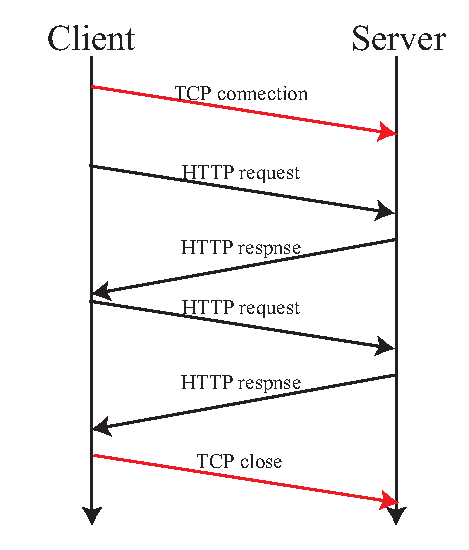
\includegraphics[width=7.5cm]{eps/HTTP.eps}
  \caption{Processing flow of general HTTP over TCP request/response}
  \label{fig:http}
\end{figure}
Fig.\ref{fig:http}に, HTTPとTCPによるWebアクセスの処理動作を示す.
Webアクセスは以下のような流れで行われる.
\begin{enumerate}
  \item 3ウェイ・ハンドシェイクによりクライアントサーバ間のTCP接続を確立する
  \item コネクションが確立すれば, クライアント側からHTTPリクエストを送る
  \item クライアントからのリクエストに対し, サーバからHTTPレスポンスが送信される
  \item クライアントがHTTPレスポンスを受け, データを受信する
  \item クライアントが要求したデータを全て受信したら, クライアント側からコネクションの切断を要求し, 切断する
\end{enumerate}
基本的に, HTTPでは, 1つのリクエストに対し, 1つのレスポンスを返す.
また, データの送受信は, 必ずクライアント側から開始されるのが, HTTPの特徴である.
TCPの主な特徴は二つある.
一つは, コネクションを確立するのに計3回のトランザクションが必要であること.
もう一つは, 1つのサーバに対して, 複数のコネクションを確立する事ができ, 効率よく通信ができるという点にある.
同時接続数は, サーバとクライアントブラウザの設定によって決められるが,
HTTP/1.1においては2以下にする事が推奨されている[\ref{HTTP/1.1}].
\subsection{HTTPパイプライン}
\begin{figure}[h]
  \centering
  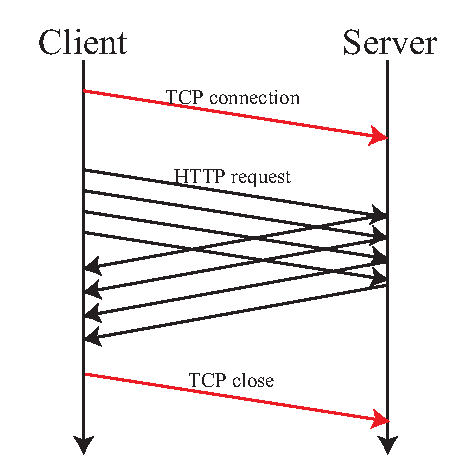
\includegraphics[width=7.5cm]{eps/HTTP_pipeline.eps}
  \caption{Processing flow of HTTP pipeline}
  \label{fig:pipeline}
\end{figure}
Fig.\ref{fig:pipeline}に, HTTPパイプラインの動作を示す.
HTTPパイプラインでは, クライアント側からの複数のHTTPリクエストが可能になる.
これにより, 通常のHTTPで生じていた次のリクエストまでの待ち時間を短縮する事ができる.
また, HTTPパイプラインでは, パイプライン化したフローは異なるプロセスでも単一のストリームとして論理的に解釈される.

\subsection{SPDY}
\begin{figure}[h]
  \centering
  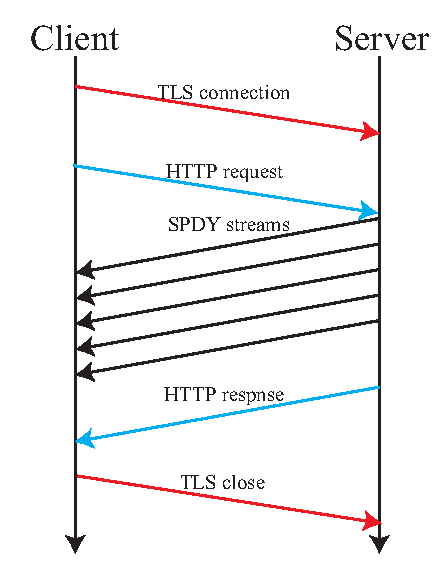
\includegraphics[width=7.5cm]{eps/server_push.eps}
  \caption{Processing flow of server push in SPDY}
  \label{fig:spdy}
\end{figure}
Fig.\ref{fig:spdy}に, SPDYのサーバプッシュ機能の動作を示す[\ref{bib:SPDY}].
SPDYは, Googleが提唱した通信プロトコルであり, TLS上で動くセッション層のプロトコルである.
TLSは, TCPの上位に位置し, 暗号通信を実現する[\ref{bib:TLS}].
このため, TCP接続のための, 3ウェイ・ハンドシェイクの他に, TLS接続のために, SSLハンドシェイクを行う必要がある.
これにより, 通常のHTTP接続よりも, 通信開始時に多くトランザクションを必要とする.

SPDYの中の高速化技術の一つでサーバプッシュがある.
サーバプッシュでは, クライアント側からHTTPリクエストを送信しなくても, サーバからデータを送信する事が可能になる.
これにより, 不要なHTTPリクエストを減らす事ができ, 全体のトランザクションの数を減らす事ができる.
さらに, SPDYではマルチストリームでデータを要求する.
このため, 複数のファイルをダウンロードする際, 複数のファイルに対し独立したストリームを生成するので,
一気にダウンロードを開始する事ができる.

\section{HTTPパイプライン, SPDYの性能評価}
本章では, HTTPパイプラインとSPDYの性能評価を示し, それらの比較を行う.
\subsection{HTTPパイプライン}
\begin{figure}[h]
  \centering
  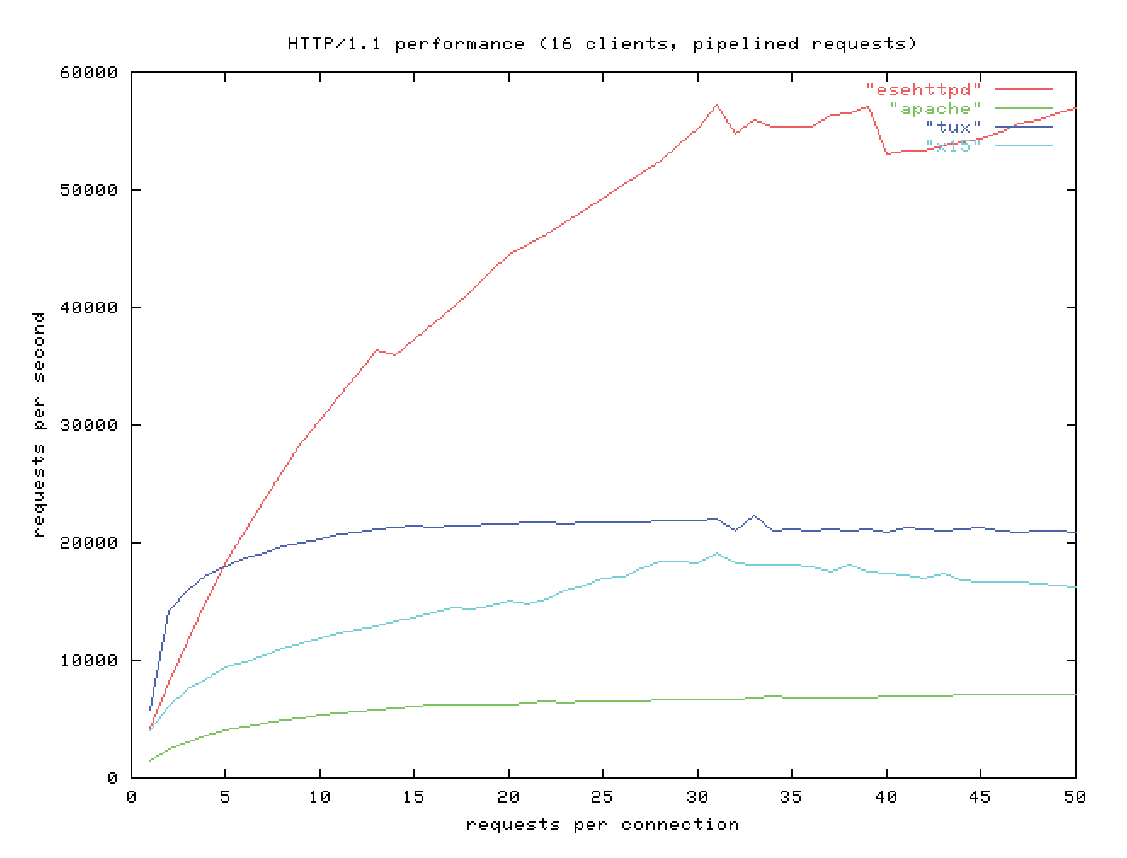
\includegraphics[width=7.5cm]{eps/pipe_graph.eps}
  \caption{Performance of HTTP pipeline On/Off}
  \label{fig:pipe_g1}
\end{figure}
Fig.\ref{fig:pipe_g1}に, HTTP/1.1のパイプライン化したリクエストを送ったときの4種類のサーバの性能を,
接続あたりのリクエスト数を変化させて測定した結果を示す[\ref{bib:Akira}].
4種のサーバの内, ``esehttpd''はHTTPパイプラインがOnになっており, それ以外はOffになっている.
また, この測定では, 非常に小さいファイル(2バイト)を転送している.
この結果から, 1秒あたりに処理できるリクエスト数が増えればその分だけパイプライン化でき,
処理できるリクエスト数が上がることが分かる.

\subsection{サーバプッシュ-SPDY}
\begin{figure}[h]
  \centering
  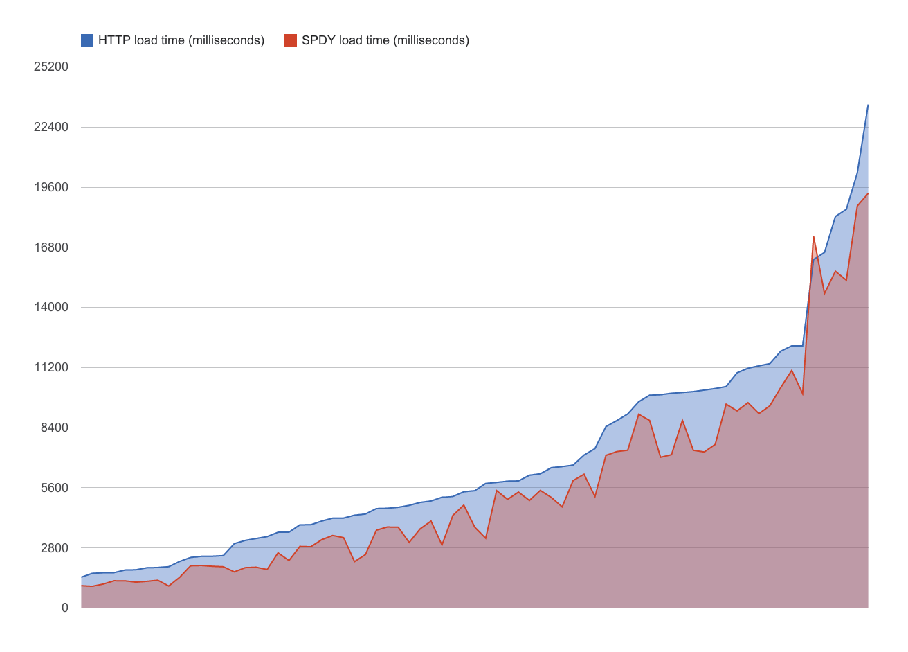
\includegraphics[width=7.5cm]{eps/SPDY_graph.eps}
  \caption{Comparison of SPDY vs. HTTP page load times}
  \label{fig:spdy_g1}
\end{figure}
\begin{figure}[h]
  \centering
  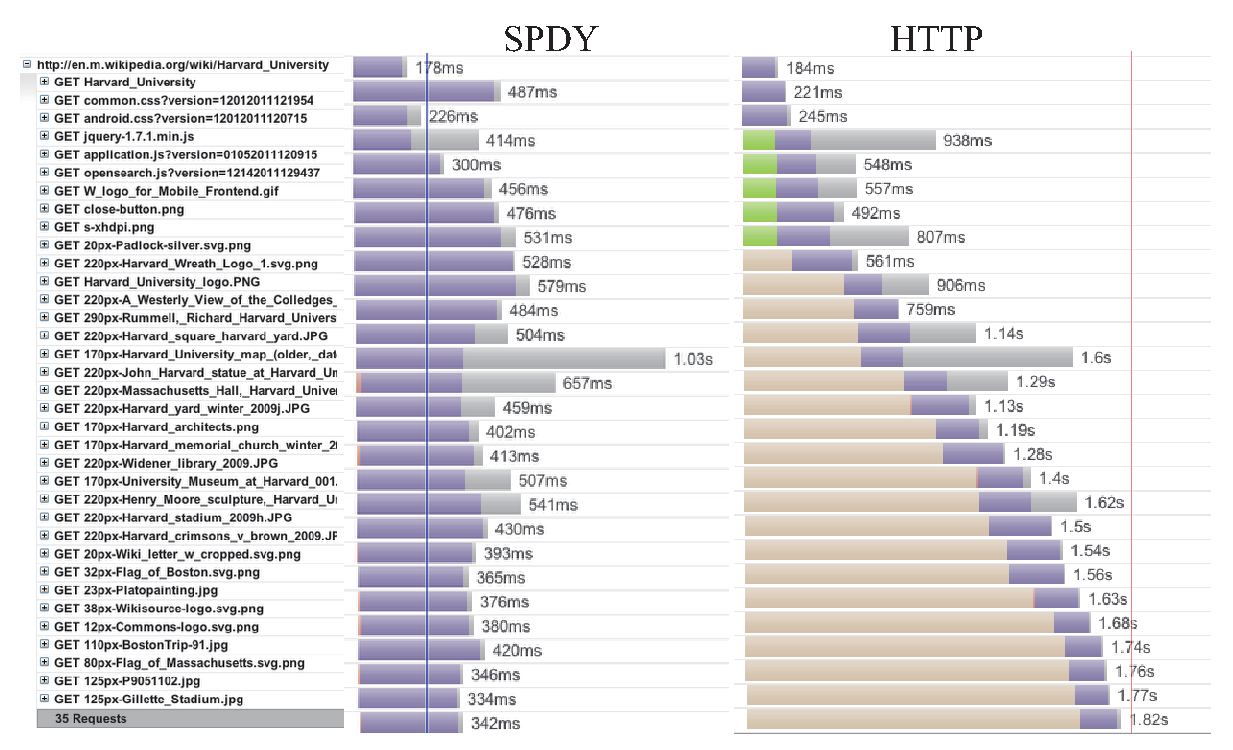
\includegraphics[width=7.5cm]{eps/SPDY_chart.eps}
  \caption{SPDY vs. HTTP load waterfall for web page of Harvard University}
  \label{fig:spdy_g2}
\end{figure}
Fig.\ref{fig:spdy_g1}に, 77個のURLに対し,
SPDYを適用した場合のページロード時間を測定した結果を示す[\ref{bib:SPDY_per}].
この測定では, 帯域を上り1[Mbps], 下り2[Mbps], RTT150[ms], パケットロス率を1\%以下,
という通信環境をエミュレートして行われた.
通常のHTTPでは, TCPコネクションを複数生成し, 並列処理としてリソースをダウンロードする.
今回の測定環境では, 最大6本までコネクションを同時接続可能だった.
その結果, Fig.\ref{fig:spdy_g2}に示すように, 6つのリソースに対しては, 同時にレスポンスを受けられるが, 残りのリソースに対しては,
リソースのダウンロードが完了するまで待つ必要がある.
一方SPDYでは, TCP接続数は1本のみだが, マルチストリームにより全てのリソースに対して, リクエストを送信する事ができる.
その結果オーバヘッドを削減でき, 平均23\%のロード時間を減少する事が可能となった.

\section{HTTPリクエスト多重化}
本章では, 1度に要求できる最大リクエスト数をそれぞれ計算し, 比較を行う.
1度に要求できる最大のリソース数は以下のように計算する事ができる.
\begin{equation}
MAX= TCP connects \times HTTP requests
\end{equation}
本稿では, この定義を用いてHTTPパイプラインとSPDYの性能を比較する.
\begin{itemize}
  \item HTTPパイプライン \\
Firefoxにおいて, HTTP/1.1に合致するサーバに対しては, TCP同時接続数は2が規定値である[\ref{bib:firefox}].
パイプラインでの最大同時リクエスト数は8となっている[\ref{bib:firefox2}].
従って, 最大のリソース数は,以下のようになる.
\begin{equation}
MAX = 2 \times 8 = 16 \nonumber
\end{equation}
  \item SPDY \\
SPDYでは, TCP接続数は1を推奨している.
また, マルチストリーム数は, デフォルトでは無制限だが, 実装では100以上に設定するように推奨している.
従って, 最大のリソース数は以下のようになる.
\begin{equation}
MAX= 1 \times 100 = 100 \nonumber
\end{equation}
\end{itemize}
上記の結果から一度に要求できる最大のリソース数は, HTTPパイプライン $<$ SPDYとなることがわかる.
さらにSPDYでは, 前述したサーバプッシュ機能により, 送るべきリクエスト数自体を減らす事ができるので,
総トランザクション数は, 上記の比較がより顕著に現れる事が期待できる.
例として, 200個のリソースに対して, 総トランザクション数を計算すると, HTTPパイプラインでは26回, SPDYでは, 3回となり,
HTTPパイプライン $>$ SPDYとなることが分かる。したがって, レスポンス時間は, HTTPパイプライン $>$ SPDYとなることが期待される.

\begin{figure}[h]
  \centering
  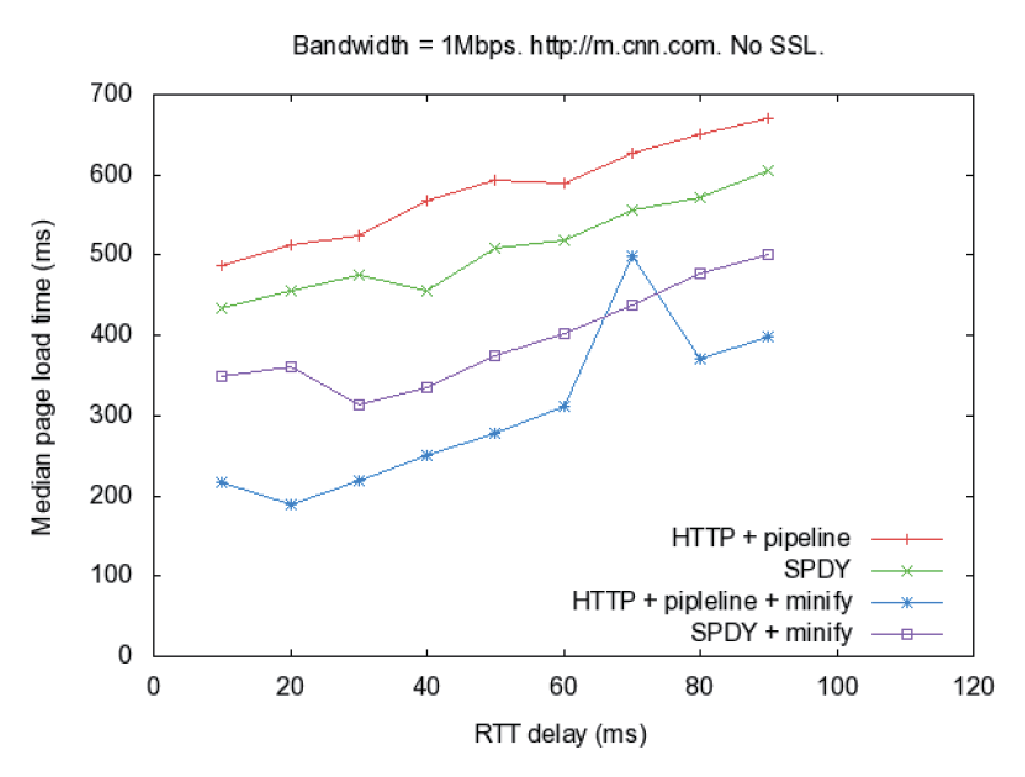
\includegraphics[width=7.5cm]{eps/compare.eps}
  \caption{Transition and forecast of the number of subscribers of Smart-Phone}
  \label{fig:compare}
\end{figure}
Fig.\ref{fig:compare}に,
CNNのモバイルサイトにアクセスした時のページロード時間を測定した結果を示す[\ref{bib:Padhye}].
このサイトには, 11個のリソース(htmlファイル1個, CSSファイル1個, imgファイル9個)があり, 計38.5[kB]のサイズである.
帯域は1[Mbps]で, HTTPパイプラインの同時接続数は11, SPDYは1という通信環境をエミュレートし, 測定された.
前述の計算よりも, HTTPパイプラインの接続数は多く設定してあるが, それでもSPDYによる通信の方がページロード時間が短縮できていることがわかる.

これらの結果から, レスポンス時間を短縮するには, 総トランザクション数に依存し, 一度に要求できるリクエスト数が多い,
またはトランザクション数を減らすことがWebアクセス高速化につながることがわかった.

\section{先行研究}

Table.\ref{tbl:trend}に近年のWebページ構成の変遷を示す[\ref{bib:http_ar}].
この統計から, 現在のWebの構成が, より多くのサーバから, より多くの重いリソースのローディングを必要としており,
そのような構成のWebページへのアクセスに対し高速化を行うことが必要となっている.
\begin{table}[!h]
\caption{The trend of Web}
\begin{tabular}{|c|c|c|}
\hline
&Nov 15 2010 & Jun 1 2013 \\ \hline \hline
Avg. Page Size & 702[kB] & 1462[kB] \\ \hline
Resources/page& 74 & 92 \\ \hline
Domain& 10 & 16 \\
\hline
\end{tabular}
\label{tbl:trend}
\end{table}

実際, SPDYでは1つのTCP接続のみ用いるため, 埋め込みデータなど, 複数のホストに対してリクエストを送る場合には, 十分効果を示さない事がある.
Table.\ref{tbl:comp}に近年報告された実際のアメリカのTOP500のWebサイトに対するSPDYの効果を示す[\ref{bib:spdy_anti}].
SPDYの仕様とこの結果から, 遅延が低い通信環境, サードパーティのドメインのような, 新たなTCP接続が必要なリソースを含むページ,
またそのリソースサイズが非常に小さいページにおいては, 効果が出にくいという事が分かる.
これは, SPDYが, TCPとSSLにより接続を確立するため, 通常のHTTPよりもトランザクション数が必要となり, 遅延が発生するである.
この事実と昨今のWebの要求条件を踏まえて, 近年報告されたSPDYを応用したWebアクセス高速化に対する先行研究を紹介する.
\begin{table}[h]
\caption{Comparison with HTTP, HTTPS, and SPDY on mobile network}
\scalebox{0.87}[1]{
\begin{tabular}{|c|c|c|}
\hline
\shortstack{Network(Down/ \\Up[kBps], Latency[ms])}&\shortstack{SPDY\\ vs.
HTTPS} & \shortstack{SPDY\\ vs.HTTP}\\ \hline \hline
\shortstack{Cable\\(5000/1000, 28)} & \shortstack{SPDY\\ 6.7\%faster}
&\shortstack{SPDY\\ 4.3\%slower}
\\
\hline \shortstack{DSL\\(1500/384, 50)} & \shortstack{SPDY\\ 4.4\%faster} &
\shortstack{SPDY\\ 0.7\%slower} \\ \hline \shortstack{Low-latancy\\(780/330,
50)} & \shortstack{SPDY\\ 3\%faster} & \shortstack{SPDY\\ 3.4\%slower} \\
\hline \shortstack{High-latency\\(780/330, 200)} & \shortstack{SPDY\\
3.7\%faster} & \shortstack{SPDY\\ 4.8\%slower} \\ \hline
\end{tabular}
}
\label{tbl:comp}
\end{table}
\subsection{BoostEdgeとSPDYによるデータとネットワークの最適化によるWebアクセス高速化技術}

\begin{figure}[h]
  \centering
  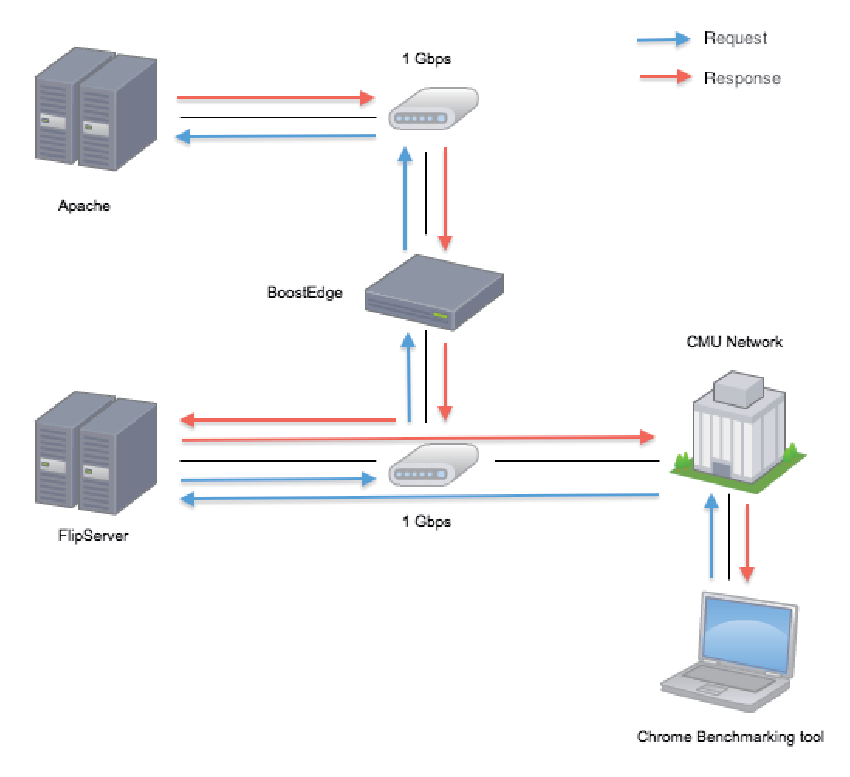
\includegraphics[width=7.5cm]{eps/BoostEdge_dia.eps}
  \caption{Dataflow for BoostEdge and SPDY combined}
  \label{fig:ongoing1}
\end{figure}

Fig.\ref{fig:pipe_g1}に, 提案されたネットワーク構成を示す[\ref{bib:boost}].
この研究では, 負荷分散のためにコンテンツ用(Apache)とトランザクション用(FlipServer)の2つのサーバを設けるような一般的な構成において,
ページロード時間を短縮を目指している.
FlipServerからApacheにリクエストを送る時に, SPDYを用いて, トランザクション数の短縮を行う.
BoostEdgeは, FlipServerとApache間のトランザクションに対して, データの最適化を行う.
最適化は主に, 頻繁にやり取りするデータのキャッシング, クライアントのスクリーンに適したサイズへの画像の非可逆圧縮を行う.
すなわち, サイズが重いファイルにはBoostEdgeが, 比較的軽い複数のファイルにはSPDYが作用する構成となっている.
このようなテストベッドにおいて, 米国で最も訪れたサイトトップ45の内, 最も多くのHTTPリクエストを必要とするサイト上位5つに対して,
そのコピーを二つのサーバに入れ, 測定を行った.
その結果をFig.\ref{fig:ongoing12}に示す.
この結果から, 単一のサーバに対する通常のHTTPと比較すると, トランザクション数が単純に増えるので, BoostEdgeの効果が出ないが,
SPDYを用いる事で, 不要なトランザクションを削減できるので, 二つのサーバをまたいで通信を行う事に対するトレードオフの影響を抑えることが可能になった.

しかしこのテストベッドでは, 一つのホストに対しリクエストを送るという点で, 現実のWebの状況を想定しているとは言えない.

\begin{figure}[h]
  \centering
  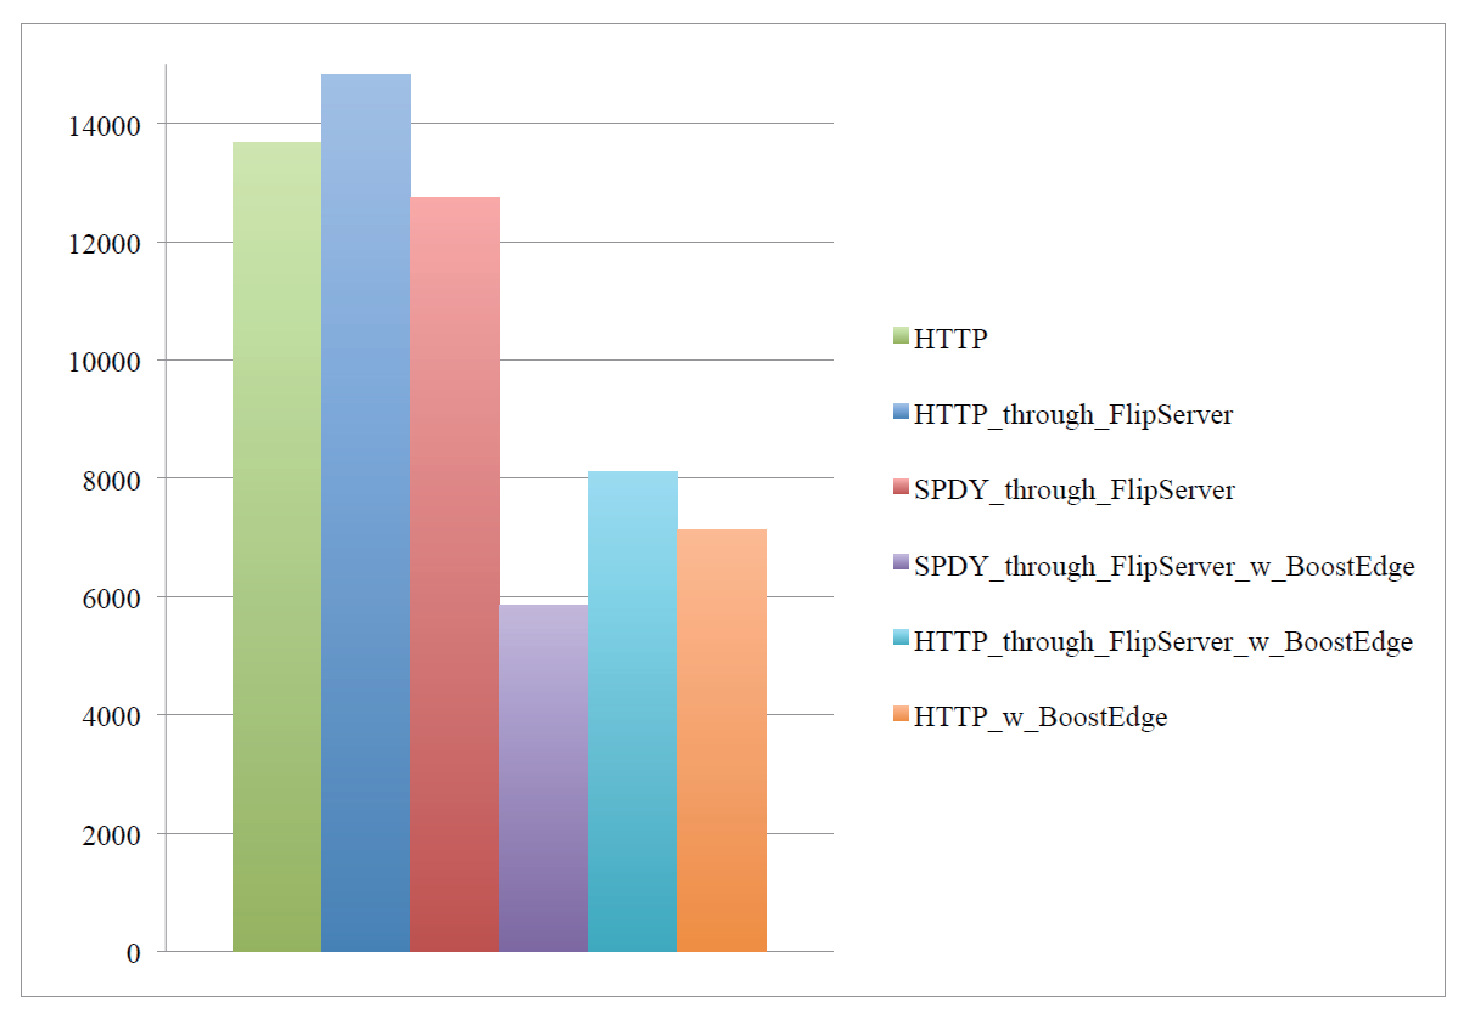
\includegraphics[width=7.5cm]{eps/BoostEdge_graph.eps}
  \caption{Results for five websites with the highest number of HTTP requests}
  \label{fig:ongoing12}
\end{figure}

\subsection{キャッシュシステムとSPDYを応用したWebアクセス高速化技術}
\begin{figure}[h]
  \centering
  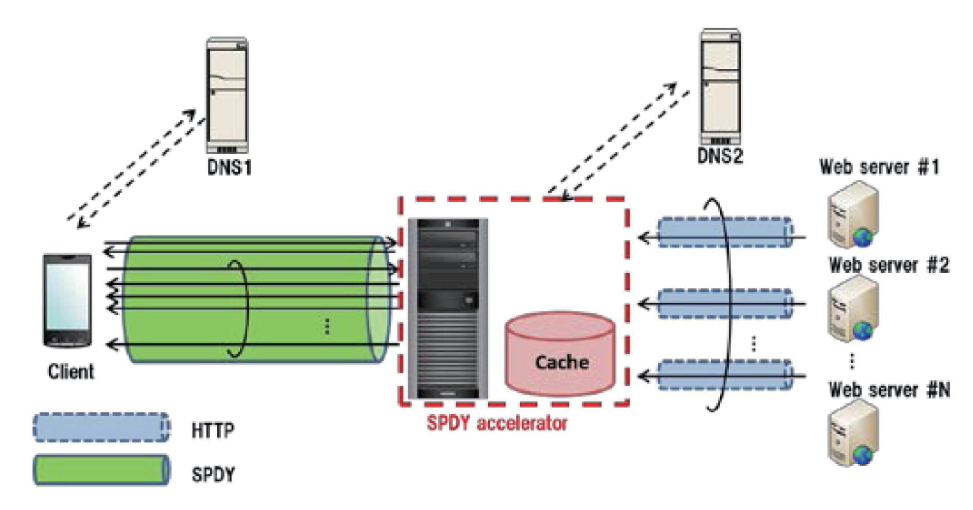
\includegraphics[width=7.5cm]{eps/http_acc_dia.eps}
  \caption{Transition and forecast of the number of subscribers of Smart-Phone}
  \label{fig:ongoing2}
\end{figure}
Fig.\ref{fig:ongoing2}に, 提案されたネットワーク構成を示す[\ref{bib:spdy_acce}].
この研究では, サードパーティからのリソースが埋め込まれたページに対して, SPDYに適したネットワークへ最適化し,
ページロード時間の短縮を目指している.
クライアントから, SPDY acceleratorに対しSPDYでリクエストを送信し, SPDY
acceleratorは対象のHTMLファイルのあるサーバへリクエストを送り, データを受信する.
SPDY acceleratorがHTMLデータを受信したら, サードパーティリソースが埋め込まれていないかチェックし, 埋め込まれていた場合は, SPDY
acceleratorがリクエストを送り, キャッシュにそのデータを保存する.
SPDY acceleratorでは, 送信可能なリソースから順次, クライアント側へレスポンスを返していく.
このシステムでは, 本来複数のサーバに対し, 複数のTCP接続が必要なため, SPDYの効果が現れにくかった構成を, クライアント側から見れば,
単一のサーバ(SPDY accelerator)にSPDYで通信を行う, と擬似的に構成することで, Webアクセスを高速化しようという試みである.
このシステムを用いて, 7つのサーバから44のリソース(HTMLファイル1, CSSファイル1,
imgファイル42), 計320[kB]に対して,
RTT150[ms]でパケットロス0\%の通信環境で, Webアクセスを行った.
その結果をFig.\ref{fig:ongoing22}に示す.
\begin{figure}[h]
  \centering
  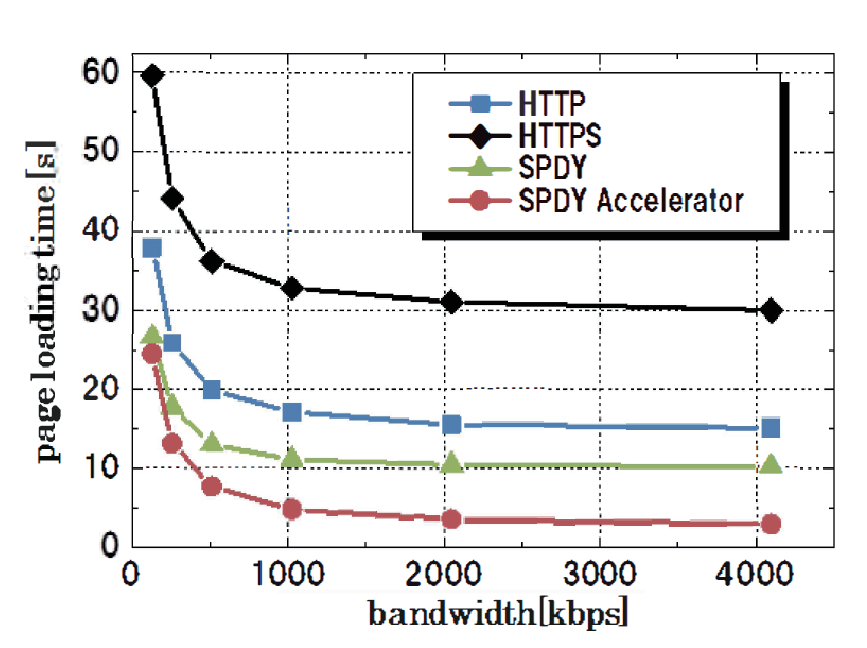
\includegraphics[width=7.5cm]{eps/http_acc_graph.eps}
  \caption{Transition and forecast of the number of subscribers of Smart-Phone}
  \label{fig:ongoing22}
\end{figure}
この結果から, 通常のHTTPを用いたものと比べ, SPDY accerelatorシステムではページロード時間を1/3に短縮する事ができた.
これにより提案手法は, マルチドメインで構成されるページ対して, SPDYを有効に作用させる事が確認できる.
今回, エミュレートした通信環境は, モバイル回線を想定したものであるが, さらにレイテンシが高い回線や,
パケットロスの多い回線に対しても有効に働くのか検討する必要がある.


これらの報告から, Webアクセス高速化のためには, 総トランザクション数を少なくすることが必要であることが確認できた.
\section{まとめ}
本稿ではWebアクセスの高速化技術を紹介した.
要求したデータに対して行われる全てのトランザクション数を算出することにより, HTTPパイプラインとSPDYのレスポンス時間を見積もり,
Webアクセスをより速くするためには, 総トランザクション数の少ない手法を使用し, ページロード時間を短縮させることが必要であることを示した.

また, 先行研究で使用されている技術がこの原則に基づいていることを確認し, 現状のWebに対するアクセス高速化のためには,
クライアント側で生成するTCPコネクションを集約することが必須であることを示した.
今後の研究動向では, レイテンシが高く, パケットロス率の高いようなモバイル通信環境において, Webアクセス高速化をどう行うべきか, という問題に対して,
いかにトランザクション数を少なくできるかという方向へ研究が進んでいくと考えられる.

\begin{thebibliography}{99}
\begin{spacing}{0.7}
\scriptsize{
\item Karl Andersson and Dan Johansson ``Mobile e-Service Using HTML5'', 37th
IEEE Conference on Local Computer Networks (LCN), 2012.
\label{bib:Karl}

\item Ngu Phuc Huy and Do vanThanh, ``Evaluation of mobile app paradigms'',
MoMM'12 10th International Conference on Advances in Mobile Computing \&
Multimedia pp25-30, 2012.
\label{bib:Ngu}

\item Eugen Pop and Victor Croitoru, ``WEB Service Based Platform for Mobile
Business'', Communications (COMM), 2012 9th International Conference pp293 -
296, June. 2012.
\label{bib:Eugen}

\item Probir Ghosh, Andrew Rau-Chaplin, ``Performance of Dynamic Web Page
Generation for Database-driven Web Sites'', IEEE NWeSP 2006. International
Conference, pp. 56-63, Sept. 2006.
\label{bib:Ghosh}

\item Peter Sevcik and Rebecca Wetzel , “Field Guide to Application Delivery Systems”, MSDN Magazine, 2006
\label{bib:Peter}

\item Z. Wang, F. X. Lin, L. Zhong, and M. Chishti. ``Why are Web Browsers Slow
on Smartphones?'', HotMobile '11, pp91-96, Mar. 2011.
\label{bib:Wang}

\item Yo Nakajima, ''スマートフォン市場規模の推移・予測(2013年3月)'',
\url{http://www.m2ri.jp/newsreleases/main.php?id=010120130328500}, Mar. 2013.
\label{bib:Nakajima}

\item Touch, Joe, John Heidemann, and Katia Obraczka. "Analysis of HTTP
performance.", ISI Research Report ISI/RR-98-463, Dec.1998.
\label{bib:Touch}

\item Raj, R. Jeberson Retna, and T. Sasipraba. "Web service selection based on
qos constraints." Trendz in Information Sciences \& Computing (TISC) IEEE, 2010.
\label{bib:Raj}

\item Raj, R. Jeberson Retna, and T. Sasipraba. "Web service selection based on
qos constraints." Trendz in Information Sciences \& Computing (TISC) IEEE, 2010.
\label{bib:Raj}

\item Bouch, Anna, M. Angela Sasse, and Hermann DeMeer. "Of packets and people:
a user-centered approach to quality of service."  8th International Workshop on.
IEEE, 2000.
\label{bib:Bouch}

\item Zona Research, "The Need for Speed II," Zona Market Bulletin, no. 5, April
2001.
\label{beb:Zona}

\item OnlineGraduatePrograms, Instant America
\url{http://www.onlinegraduateprograms.com/instant-america/}, March 2012.
\label{bib:Instant}

\item Junichi Funasaka, ``高ロス率ネットワークにおける分割ダウンロードの性能向上を目指すトランスポートプロトコルについての一検討'',
201th IEICE Technical Report pp.253-258, 2008.
\label{bib:Junichi}

\item Huang, Junxian, et al. "Anatomizing application performance differences on
smartphones." Proceedings of the 8th international conference on Mobile systems, applications, and services. ACM, 2010.
\label{bib:Huang}

\item Sevani, Vishal, and Bhaskaran Raman. "Understanding HTTP traffic
performance in TDMA mesh networks." Communication Systems and Networks (COMSNETS), 2013 Fifth International Conference on. IEEE, 2013.
\label{bib:Sevani}

\item Natarajan, Preethi, et al. "SCTP: an innovative transport layer protocol
for the web." Proceedings of the 15th international conference on World Wide Web. ACM, 2006.
\label{bib:Natarajan}

\item Radhakrishnan, Sivasankar, et al. "TCP fast open." Proceedings of the
Seventh COnference on emerging Networking EXperiments and Technologies. ACM, 2011.
\label{bib:Radhakrishnan}

\item Dukkipati, Nandita, et al. "An argument for increasing TCP’s initial
congestion window." ACM SIGCOMM Computer Communication Review 40.3 (2010): 27-33.
\label{bib:Dukkipati}

\item Agarwal, Sachin. "Real-time web application roadblock: Performance penalty
of HTML sockets." Communications (ICC), 2012 IEEE International Conference on. IEEE, 2012.
\label{bib:Agarwal}

\item Xinogalos, Stelios, Kostas E. Psannis, and Angelo Sifaleras. "Recent
advances delivered by HTML 5 in mobile cloud computing applications: a survey." Proceedings of the Fifth Balkan Conference in Informatics. ACM, 2012.
\label{bib:Xinogalos}

\item Cohen, Edith, and Haim Kaplan. "Prefetching the means for document
transfer: A new approach for reducing Web latency." Computer Networks 39.4 (2002): 437-455.
\label{bib:Edith}

\item Al-Fares, Mohammad, et al. "Overclocking the Yahoo!: CDN for faster web
page loads." Proceedings of the 2011 ACM SIGCOMM conference on Internet measurement conference. ACM, 2011.
\label{bib:Mohammad}

\item Fielding, R., et al. "RFC 2616: Hypertext Transfer Protocol–HTTP/1.1,
1999." URL http://www. rfc. net/rfc2616. html (2009).
\label{HTTP/1.1}

\item Belshe, Mike, and Roberto Peon. "SPDY Protocol." (2012).
\label{bib:SPDY}

\item Dierks, T., and E. Rescorla. "Rfc 5246: The transport layer security
(tls) protocol." The Internet Engineering Task Force (2008).
\label{bib:TLS}

\item Akira Higuchi, ``Getting High Performance With Esehttpd'',
\url{http://esehttpd.sourceforge.jp/doc/ja/high-performance.html}
\label{bib:Akira}

\item Matt Welsh, Ben Greenstein, and Michael Piatek, ``SPDY Performance on
Mobile Networks'',
\url{https://developers.google.com/speed/articles/spdy-for-mobile}, April. 2012.
\label{bib:SPDY_per}

\item Darin Fisher, ``HTTP Pipelining FAQ'',
\url{https://developer.mozilla.org/en-US/docs/HTTP_Pipelining_FAQ}, 2010.
\label{bib:firefox}

\item  Firefox and Hacks, ``The Truth About the Firefox “Pipelining” Trick'',
\url{http://egonitron.com/2007/05/25/the-truth-about-the-firefox-pipelining-trick/},
2007.
\label{bib:firefox2}

\item Padhye, Jitu. "A comparison of SPDY and HTTP performance." (2012).
\label{bib:Padhye}

\item ``HTTP Archive'', \url{http://httparchive.org/}, June. 2013.
\label{bib:http_ar}

\item Guy Podjarmy, ``Not as SPDY as You Thought'',
\url{http://www.guypo.com/technical/not-as-spdy-as-you-thought/}, June. 2012.
\label{bib:spdy_anti}

\item Rosenberg, Steven, Surbhi Dangi, and Isuru Warnakulasooriya. "Data and
Network Optimization Effect on Web Performance." (2012).
\label{bib:boost}

\item Gen Mineki, Satoshi Uemura, and Teruyuki Hasegawa, ``SPDY Accelerator
for Improving Web Access Speed'', ICACT 2013, Jan. 2013.
\label{bib:spdy_acce}



}
\end{spacing}
\end{thebibliography}

\end{document}